\begin{frame}{Mô tả dữ liệu và bài toán}
    Trong báo cáo này, nhóm sử dụng bộ dữ liệu của một công ty do Giảng viên TS. Nguyễn Thị Ngọc Anh cung cấp. Bộ dữ liệu này gồm 2 file excel:
\begin{itemize}
    \item SP\_Plan: Kế hoạch bán sản phẩm A, B1, B2 trong 12 quý, từ 2021 đến 2023.
    \item SP\_DoiThu: Kế hoạch bán sản phẩm bao gồm cả lượng và giá trị của A, B, C trong 46 tháng, từ 1/2020 đến 10/2023.
\end{itemize}

Bài toán dự báo kế hoạch 1-4 quý tiếp theo của từng sản phẩm A, B1, B2.
    
\end{frame}

\begin{frame}{Mô tả dữ liệu và bài toán}
    \begin{figure}[H]
    \centering
    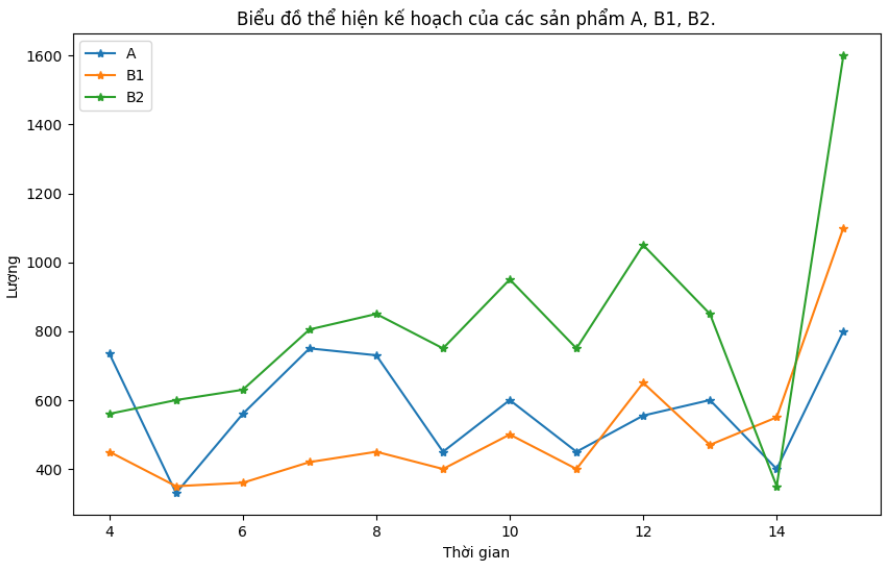
\includegraphics[width = 0.8\textwidth]{figure/AB1B2.png}
    \caption{Biểu đồ thể hiện số lượng của sản phẩm A, B1, B2 theo quý.}
    \label{fig:AB1B2}
\end{figure}
\end{frame}

\begin{frame}{Mô tả dữ liệu và bài toán}
    \begin{figure}[H]
    \centering
    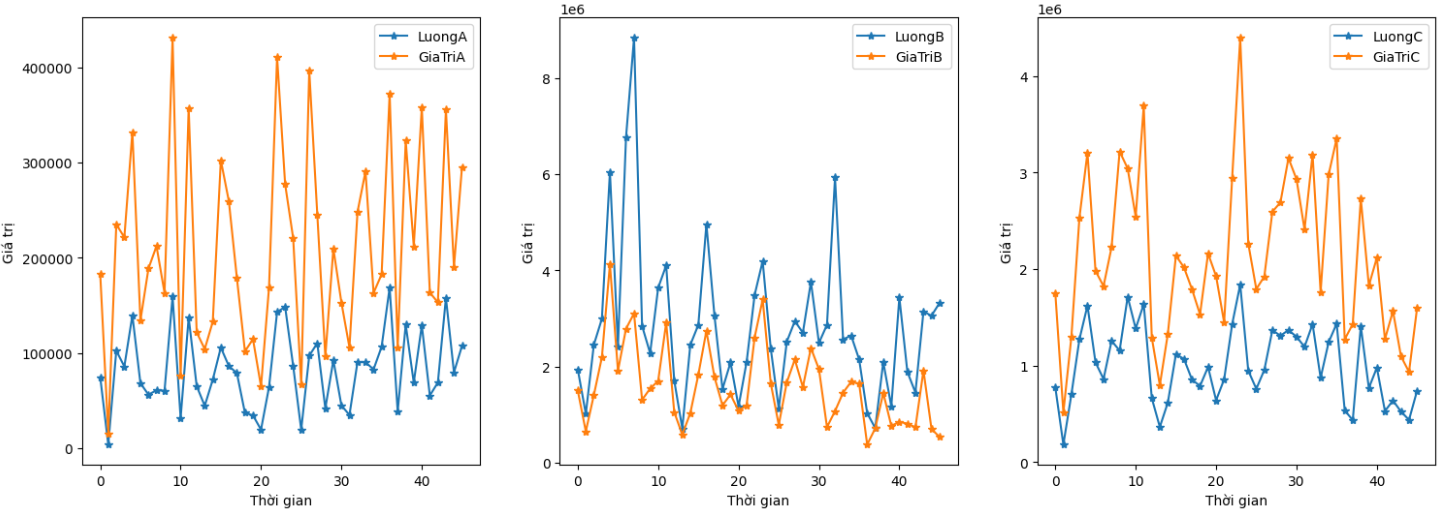
\includegraphics[width = 0.9\textwidth]{figure/ABCGiaTriLuong.PNG}
    \caption{Biểu đồ thể hiện sản phẩm A, B, C đối thủ theo tháng.}
    \label{fig:ABCGiaTriLuong}
\end{figure}
\end{frame}

\begin{frame}{Xử lý dữ liệu}
    Do kế hoạch bên công ty là theo quý, còn đối thủ là theo tháng. Do đó gộp 3 tháng làm 1 quý và bỏ đi phần kế hoạch năm 2020 và tháng 10/2023 của đối thủ, quý 4 năm 2023 của công ty. Bỏ đi kế hoạch của sản phẩm C, và chỉ lấy phần lượng của mỗi sản phẩm A, B. Còn lại thu được 11 quý từ quý 1/2021 đến quý 3/2023. 

    \begin{figure}[H]
    \centering
    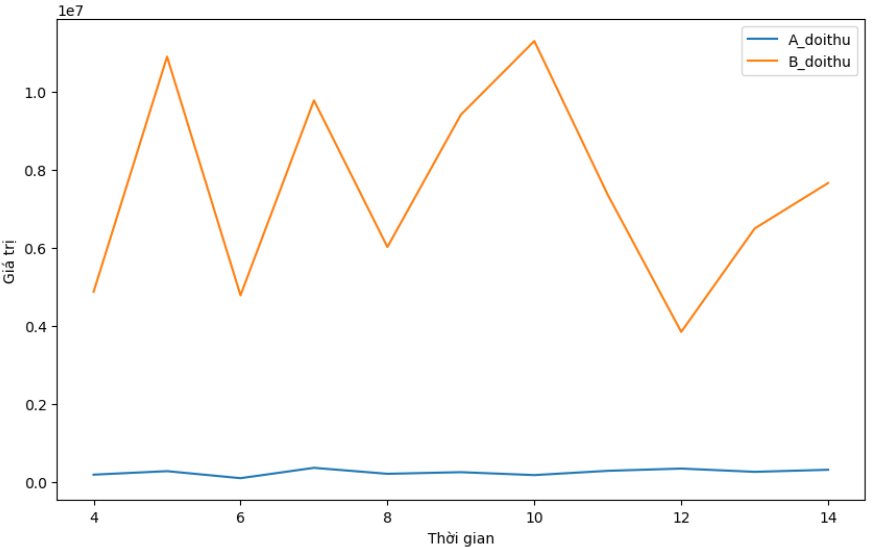
\includegraphics[width = 0.7\textwidth]{figure/ABLuong.PNG}
    \caption{Biểu đồ thể hiện sản phẩm A, B của đối thủ theo quý.}
    \label{fig:ABLuong}
\end{figure}

\end{frame}


\begin{frame}{Xây dựng mô hình}
    Nhóm chia dữ liệu thành 2 tập train và test với train gốm 7 quý đầu, test gồm 4 quý sau. Và xây dựng, thử nghiệm các mô hình sau:
\begin{itemize}
    \item Sử dụng với 2 trường A, A đối thủ: VAR - OLS, VAR - Durbin-Levinson.
    \item Sử dụng với 3 trường B1, B2, B đối thủ: VAR - OLS, VAR - Durbin-Levinson.
    \item Sử dụng 5 trường A, B1, B2, A đối thủ, B đối thủ: VAR - OLS, VAR - Durbin-Levinson, Holt-Winter tối ưu theo Log-Likelihood, Holt-Winters tối ưu theo MSE.
\end{itemize}
\end{frame}

\begin{frame}{Kết quả thực nghiệm}
    Qua quá trình thử nghiệm, nhóm sử dụng độ đo MAE thu được kết quả đánh giá sau:

    \begin{table}[H]
    \centering
    \resizebox{\textwidth}{!}{ 
        \begin{tabular}{|c|c|c|c|c|c|c|c|c|c|c|}
        \hline
            \multirow{2}{*}{Mô hình} & \multicolumn{2}{c|}{A và A đối thủ} & \multicolumn{3}{c|}{B1, B2 và B đối thủ} & \multicolumn{5}{c|}{A, B1, B2, A đối thủ và B đối thủ} \\ \cline{2-11}
            & A & A đối thủ & B1 & B2  & B đối thủ & A & B1 & B2 & A đối thủ & B đối thủ \\ \hline
            VAR - OLS & \textbf{63.608} & 99694.263 & \textbf{97.616} & 328.073 & 6814639.757 & 163.212 & 97.505 & 327.786 & \textbf{41173.739} & 6811127.587 \\ \hline
            VAR - Durbin-Levinson & 111.328 & \textbf{74709.311} & 114.633 & \textbf{219.033} & \textbf{1928826.146} & \textbf{103.498} & 102.971 & \textbf{156.071} & 60742.338 & \textbf{2158559.805} \\ \hline
            Holt-Winter tối ưu theo Log-likelihood & & & & & & 245.501 & \textbf{57.501} & 339.251 & 97291.501 & 4844239.125 \\ \hline
            Holt-Winter tối ưu theo MSE & & & & & & 316.328 & 98.033 & 354.922 & 82337.041 & 9509946.258 \\ \hline
        \end{tabular}
    }
\end{table}
\end{frame}

\begin{frame}{Mô hình VAR - OLS}
    \begin{table}[H]
    \centering
    \caption{Kết quả dự báo 4 quý năm 2024 bằng mô hình VAR - OLS.}
    \label{DB4nam2024}
    \resizebox{\textwidth}{!}{ 
        \begin{tabular}{|c|c|c|c|c|c|c|c|c|c|c|}
        \hline
            \multirow{2}{*}{Quý} & \multicolumn{2}{c|}{A và A đối thủ} & \multicolumn{3}{c|}{B1, B2 và B đối thủ} & \multicolumn{5}{c|}{A, B1, B2, A đối thủ và B đối thủ} \\ \cline{2-11}
            & A & A đối thủ & B1 & B2  & B đối thủ & A & B1 & B2 & A đối thủ & B đối thủ \\ \hline
            1 & 501.369 & 430125.909 & 480.701 & 835.505 & 4878039.48 & 477.249 & 480.841 & 835.488 & 272521.765 & 4880684.39 \\ \hline
            2 & 704.477 & 384310.265 & 480.906 & 671.971 & 4877756.56& 438.670 & 481.041 & 672.221 & 259961.421 & 4880244.12 \\ \hline
            3 & 611.613 & 386588.924 & 431.586  & 443.055 & 4813185.67 & 345.854 & 431.746 & 443.405 & 233389.177 & 4817447.48 \\ \hline
            4 & 638.573 & 429640.797 & 352.013  & 451.676 & 4893416.66 & 335.253 & 352.348 & 451.911 & 203718.448 & 4897584.47 \\ \hline
        \end{tabular}
     }
\end{table}
\end{frame}

\begin{frame}{Mô hình VAR - OLS}
\begin{figure}[H]
    \centering
    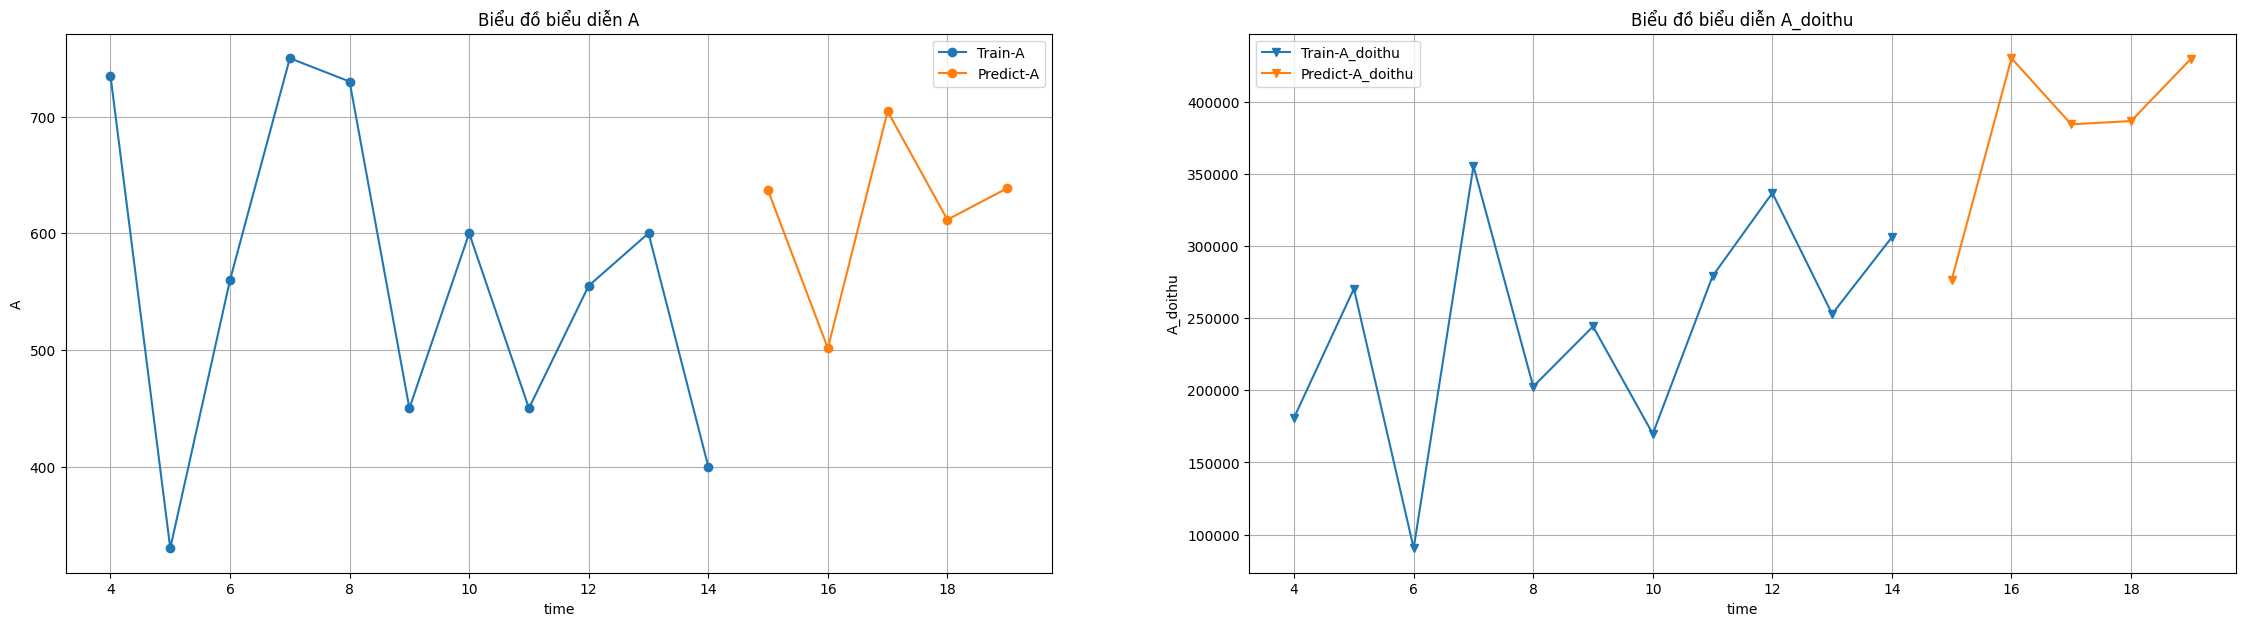
\includegraphics[width = \textwidth]{figure/VAR2.png}
    \caption{Dự đoán 4 quý năm 2024 của mô hình VAR - OLS trên 2 trường A và A đối thủ.}
    \label{fig:var2}
\end{figure}
\end{frame}


\begin{frame}{Mô hình VAR - OLS}
\begin{figure}[H]
    \centering
    \includegraphics[width = \textwidth]{figure/VAR3.png}
    \caption{Dự đoán 4 quý năm 2024 của mô hình VAR - OLS trên 3 trường B1, B2 và B đối thủ.}
    \label{fig:var2}
\end{figure}
\end{frame}

\begin{frame}{Mô hình VAR - OLS}
    \begin{figure}[H]
    \centering
    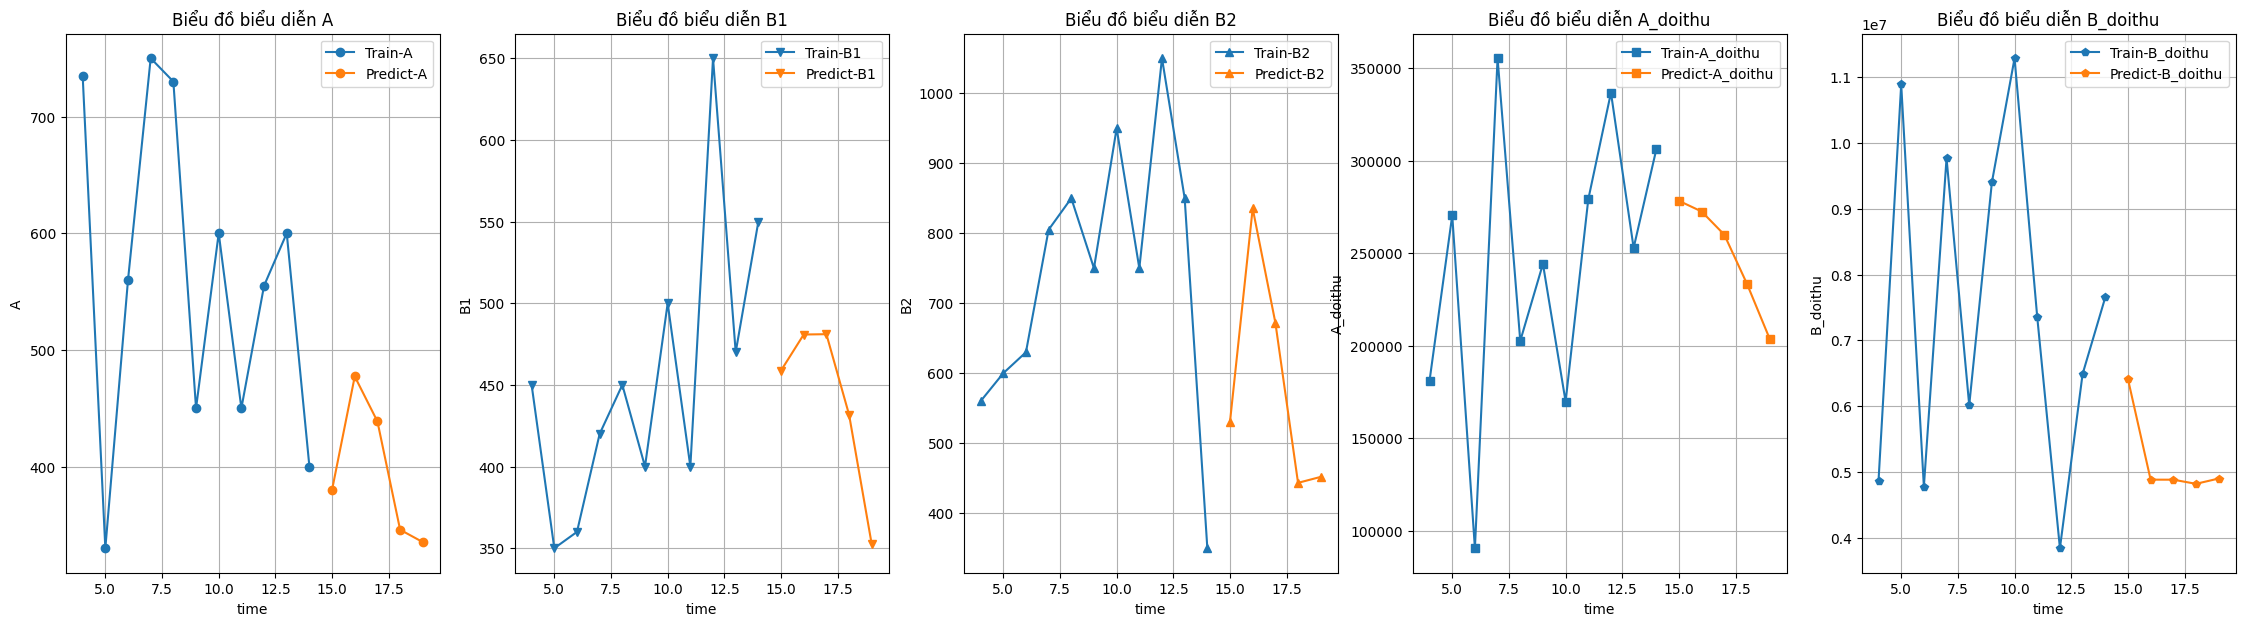
\includegraphics[width = \textwidth]{figure/dudoanVAR.png}
    \caption{Dự đoán 4 quý năm 2024 tiếp theo của mô hình VAR - OLS trên cả 5 trường.}
    \label{fig:var5}
\end{figure}
\end{frame}

\begin{frame}{Mô hình VAR - Durbin-Levinson}
    \begin{table}[H]
    \centering
    \caption{Kết quả dự báo 4 quý năm 2024 bằng mô hình VAR - Durbin-Levinson.}
    \label{DB4nam2024}
    \resizebox{\textwidth}{!}{ 
        \begin{tabular}{|c|c|c|c|c|c|c|c|c|c|c|}
        \hline
            \multirow{2}{*}{Quý} & \multicolumn{2}{c|}{A và A đối thủ} & \multicolumn{3}{c|}{B1, B2 và B đối thủ} & \multicolumn{5}{c|}{A, B1, B2, A đối thủ và B đối thủ} \\ \cline{2-11}
            & A & A đối thủ & B1 & B2  & B đối thủ & A & B1 & B2 & A đối thủ & B đối thủ \\ \hline
            1 & 534.637 & 260718.824 & 456.899 & 757.619 & 8020657.233 & 529.176 & 458.487 & 760.954 & 271257.466  & 7956737.484 \\ \hline
            2 & 572.094 & 236579.687 & 453.417 & 734.091 & 7291676.408 & 580.709 & 460.710 & 747.793 & 229189.165 & 7025864.153 \\ \hline
            3 & 554.189 & 248210.334 & 454.772 & 741.086 & 7565733.786 & 540.675 & 451.292 & 741.719 & 258889.882 & 7832721.811  \\ \hline
            4 & 562.794 & 242614.486 & 454.436 & 740.095 & 7451979.116 & 575.599 & 457.979 & 741.555 & 232923.170 & 7195879.347 \\ \hline
        \end{tabular}
    }
\end{table} 
\end{frame}

\begin{frame}{Mô hình VAR - Durbin-Levinson}
    \begin{figure}[H]
    \centering
    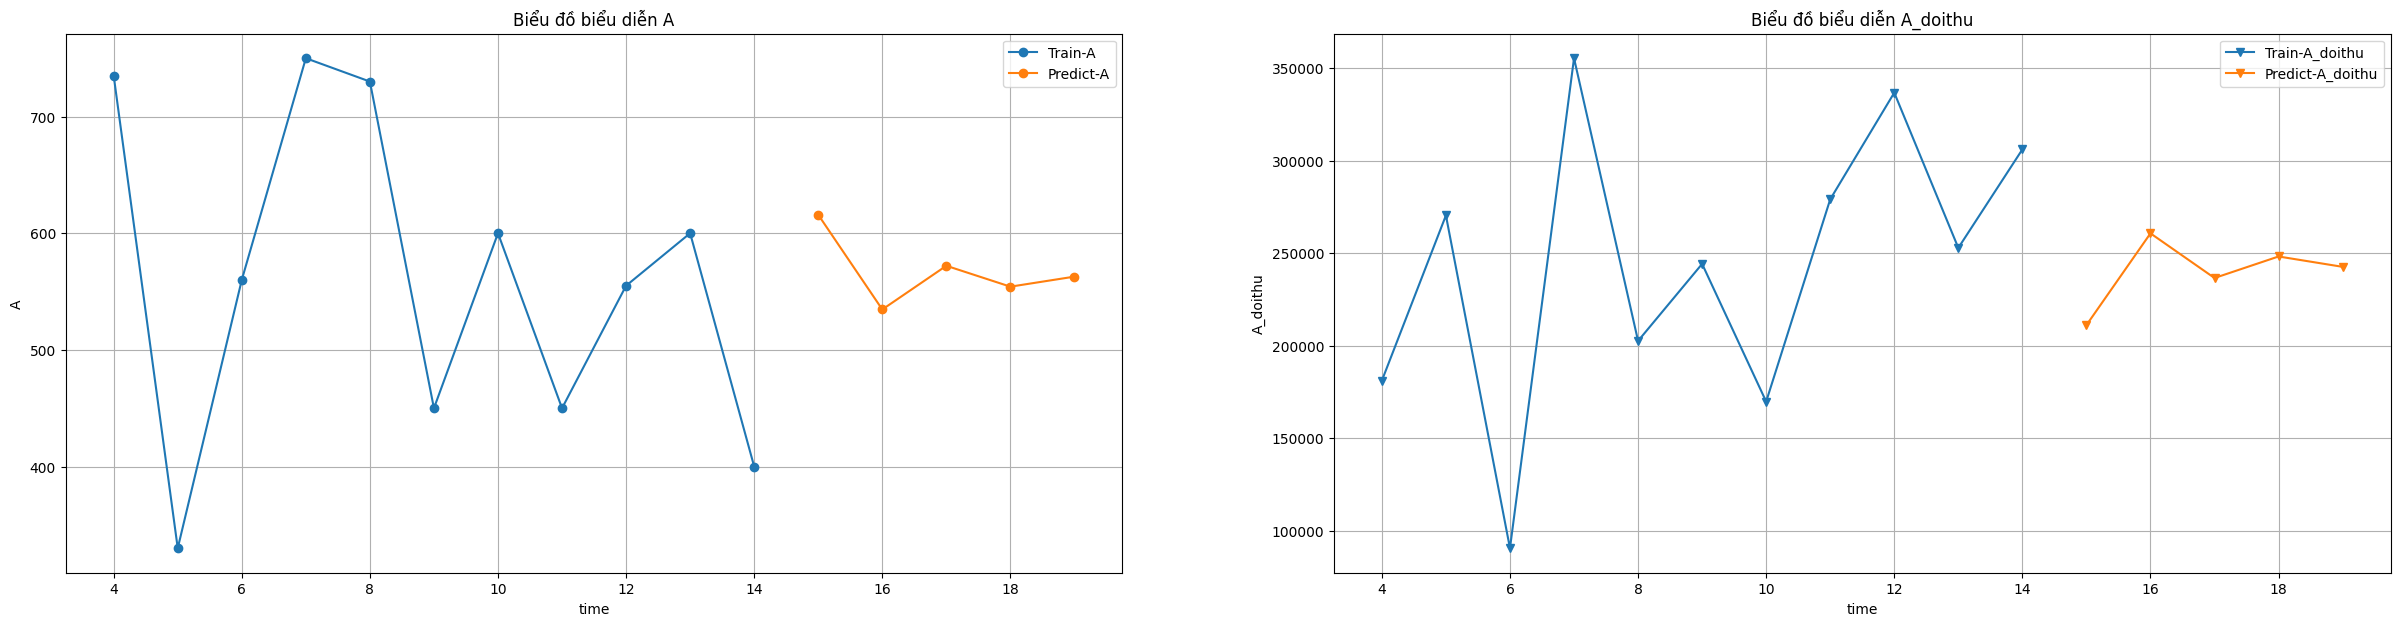
\includegraphics[width = \textwidth]{figure/preDB2.png}
     \caption{Kết quả dự đoán các quý tiếp theo của mô hình VAR - Durbin-Levinson trên 2 trường A và A đối thủ.}
\end{figure}
\end{frame}

\begin{frame}{Mô hình VAR - Durbin-Levinson}
    \begin{figure}[H]
    \centering
    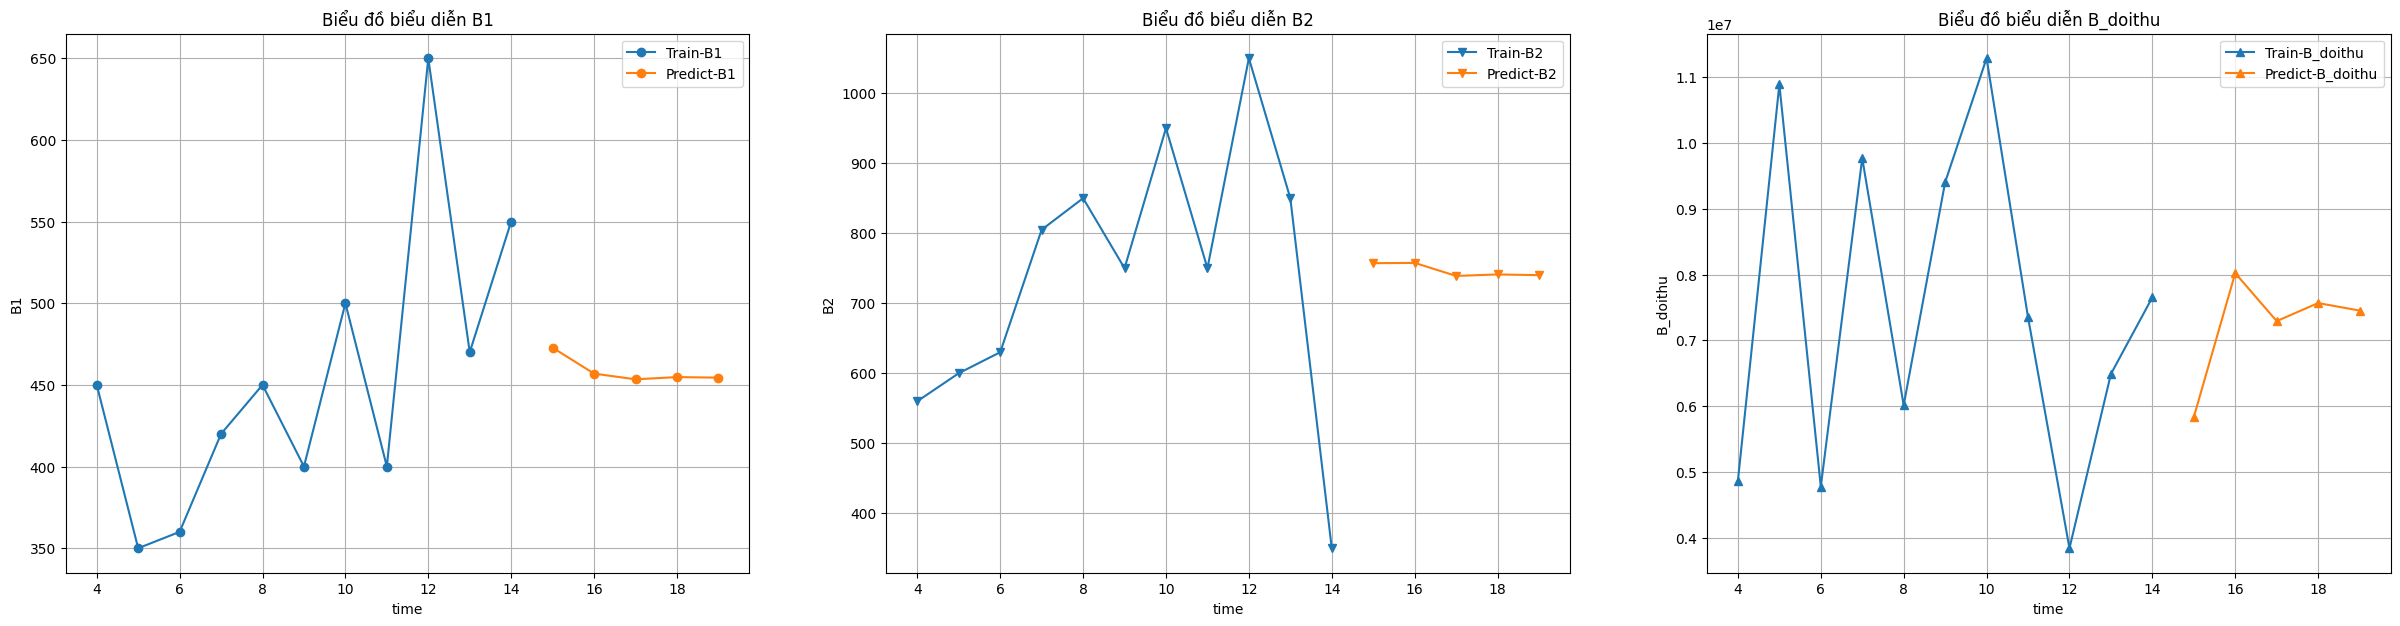
\includegraphics[width = \textwidth]{figure/preDB3.png}
     \caption{Kết quả dự đoán các quý tiếp theo của mô hình VAR - Durbin-Levinson trên 3 trường B1, B2 và B đối thủ.}
\end{figure}
\end{frame}

\begin{frame}{Mô hình VAR - Durbin-Levinson}
    \begin{figure}[H]
    \centering
    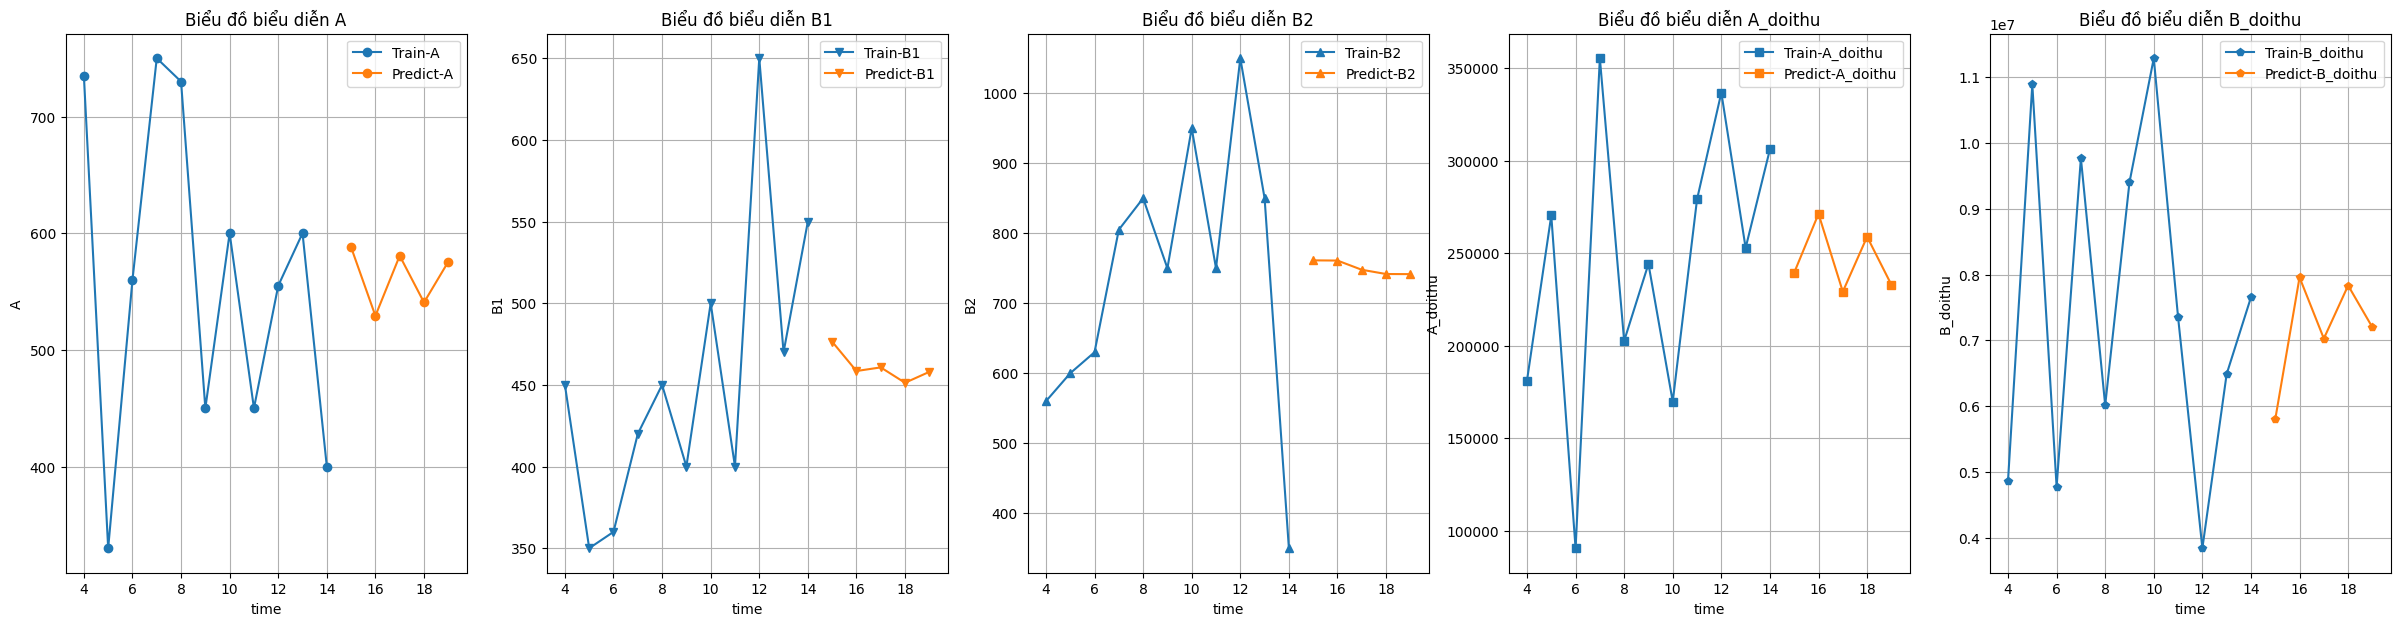
\includegraphics[width = \textwidth]{figure/preDB5.png}
     \caption{Kết quả dự đoán các quý tiếp theo của mô hình VAR - Durbin-Levinson trên cả 5 trường.}
\end{figure}
\end{frame}

\begin{frame}{Mô hình Holt-Winters tối ưu theo hàm Log-Likelihood}
    \begin{table}[H]
    \centering
    \caption{Kết quả dự báo 4 quý năm 2024 bằng mô hình Holt-Winters tối ưu theo hàm Log-Likelihood.}
    \label{HL4nam2024}
    \resizebox{\textwidth}{!}{ 
        \begin{tabular}{|c|c|c|c|c|c|}
        \hline
         Quý & A & B1 & B2 & A đối thủ & B đối thủ  \\ \hline
         1 & 611.179 & 667.743 & 945.461 & 337227.027 & 3748242.589 \\ \hline
         2 & 398.308 & 557.512 & 858.160 & 352909.032 & 7769289.737 \\ \hline
         3 & 458.769 & 620.615 & 767.525 & 285877.371 & 6748481.551 \\ \hline
         4 & 522.308 & 598.846 & 934.326 & 438602.865 & 7113320.903 \\ \hline
        \end{tabular}
    }
\end{table}
\end{frame}

\begin{frame}{Mô hình Holt-Winters tối ưu theo hàm Log-Likelihood}
    \begin{figure}[H]
    \centering
    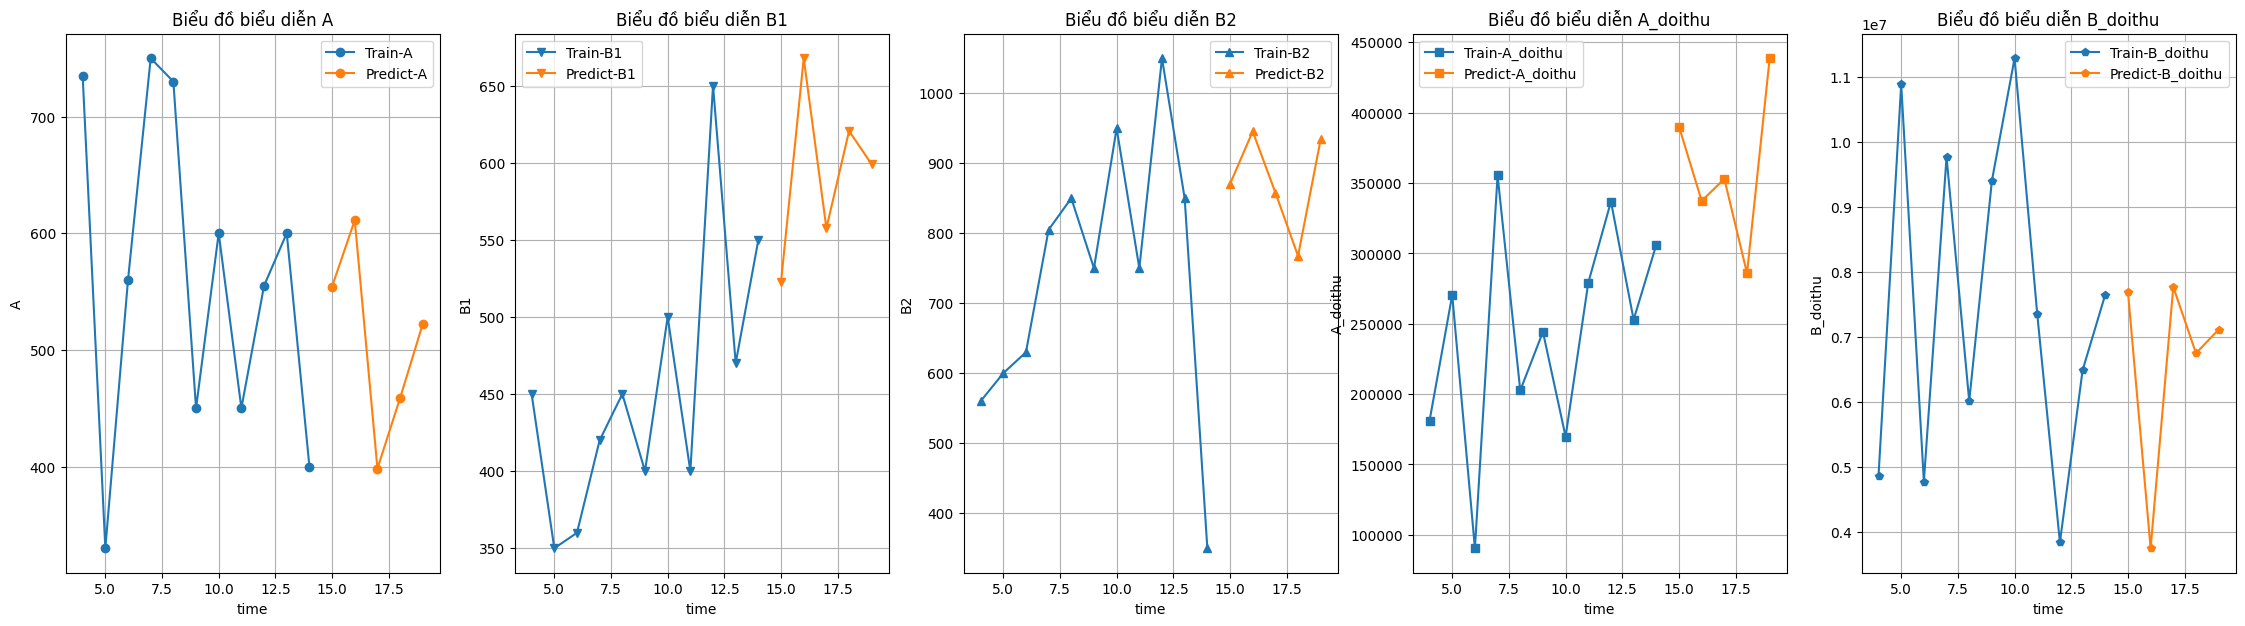
\includegraphics[width = \textwidth]{figure/HW-likelihood.png}
     \caption{Kết quả dự đoán 4 quý năm 2024 bằng mô hình Holt-Winters tối ưu theo hàm Likelihood.}
\end{figure}
\end{frame}

\begin{frame}{Mô hình Holt-Winters tối ưu theo hàm MSE}
    \begin{table}[H]
    \centering
    \caption{Kết quả dự báo 4 quý năm 2024 bằng mô hình Holt-Winters tối ưu theo hàm MSE.}
    \label{HM4nam2024}
    \resizebox{\textwidth}{!}{ 
        \begin{tabular}{|c|c|c|c|c|c|}
        \hline
         Quý & A & B1 & B2 & A đối thủ & B đối thủ  \\ \hline
         1 & 783.931 & 782.078 & 1181.535 & 408328.905 & 6563700.954 \\ \hline
         2 & 549.187 & 671.608 & 1103.708 & 431537.413 & 10697519.506 \\ \hline
         3 & 623.912 & 726.248 & 1034.390 & 354718.765 & 9344292.680 \\ \hline
         4 & 741.065 & 751.774 & 1263.108 & 541828.309 & 10713969.767 \\ \hline
        \end{tabular}
    }   
\end{table} 
\end{frame}

\begin{frame}{Mô hình Holt-Winters tối ưu theo hàm MSE}
    \begin{figure}[H]
    \centering
    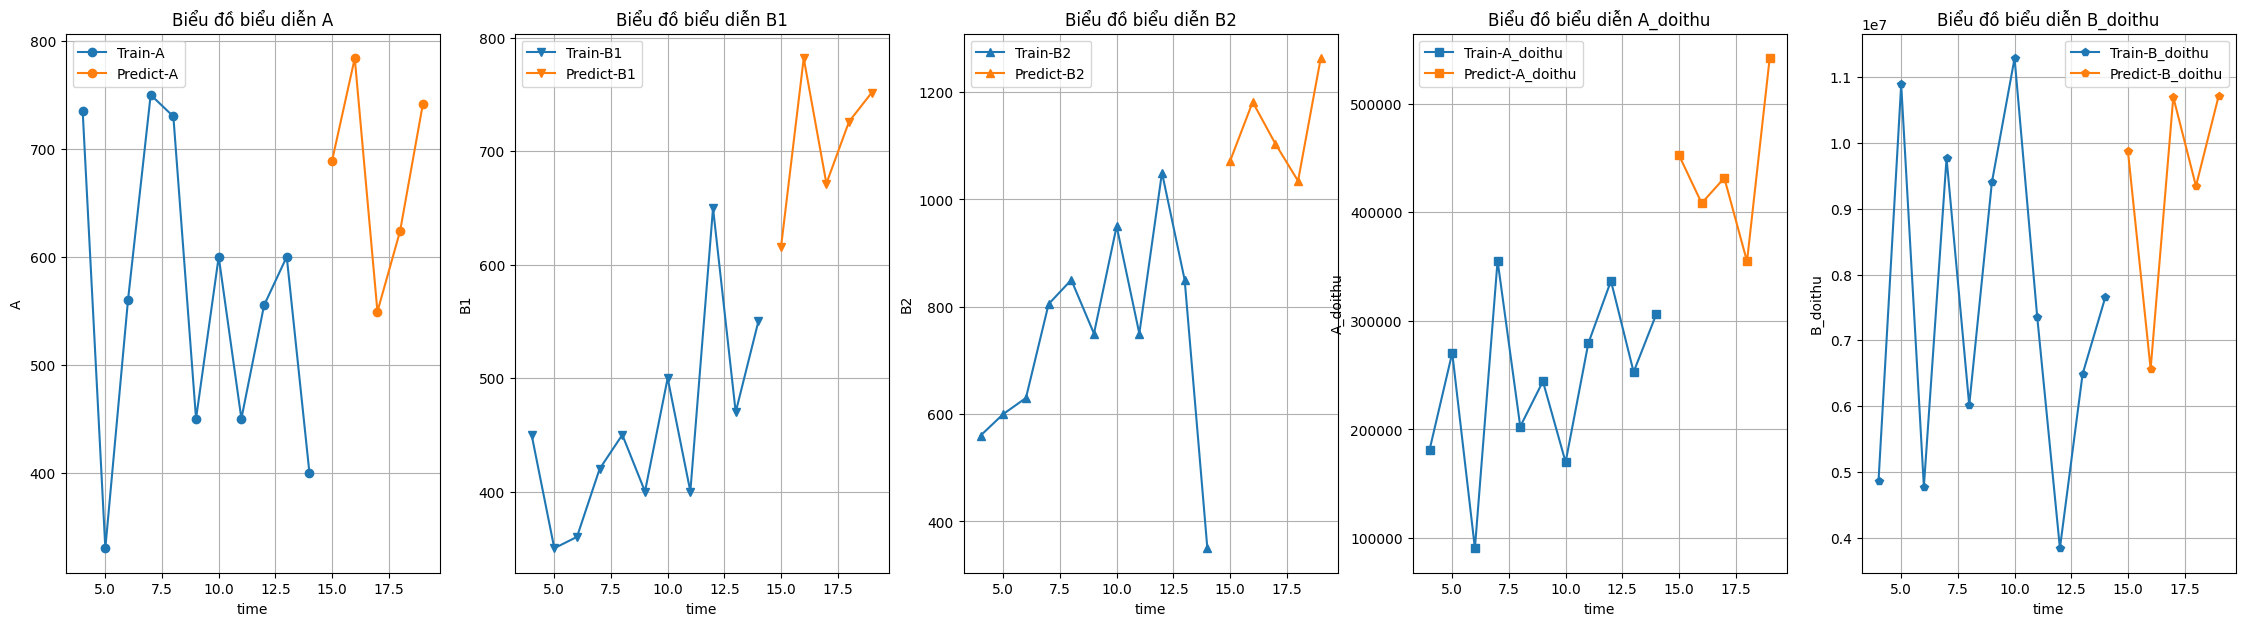
\includegraphics[width = \textwidth]{figure/HW-mse.png}
    \caption{Kết quả dự báo 4 quý năm 2024 bằng mô hình Holt-Winters tối ưu theo hàm MSE.}
\end{figure}
\end{frame}